\documentclass[a4paper,11pt,french]{article}
\usepackage[utf8]{inputenc}

\usepackage[T1]{fontenc}
\usepackage[francais]{babel} 
\usepackage[top=2cm, bottom=2cm, left=2cm, right=2cm, includeheadfoot]{geometry} %pour les marges
\usepackage{lmodern}
\usepackage{pict2e}
\usepackage{tikz}	
\usepackage{tikz-uml}
\usepackage{fancyhdr} % Required for custom headers
\usepackage{lastpage} % Required to determine the last page for the footer
\usepackage{extramarks} % Required for headers and footers
\usepackage{graphicx} % Required to insert images
\usepackage{tabularx, longtable}
\usepackage{color, colortbl}
\usepackage{lscape}
%\usepackage[hidelinks]{hyperref}
\usepackage{longtable}
\usepackage{multirow}
\usepackage{rotating}
\usepackage{gensymb}


\usepackage{algorithm}
\usepackage{algorithmic}


\usepgflibrary{arrows} % for pgf-umlsd

\usetikzlibrary{trees,shapes.geometric,arrows,decorations.pathmorphing,backgrounds,fit,positioning,shapes.symbols,chains	}

\linespread{1.1} % Line spacing

% Set up the header and footer
\pagestyle{fancy}
\lhead{\textbf{\hmwkClass -- \hmwkSubject \\ \hmwkTitle \\ \hmwkDocName}} % Top left header
\rhead{
\includegraphics[width=10em]{logo_univ.png}}
\lfoot{\lastxmark} % Bottom left footer
\cfoot{} % Bottom center footer
\rfoot{Page\ \thepage\ / \pageref{LastPage}} % Bottom right footer
\renewcommand\headrulewidth{0.4pt} % Size of the header rule
\renewcommand\footrulewidth{0.4pt} % Size of the footer rule

\setlength{\headheight}{40pt}

\newcommand{\hmwkTitle}{\'Etude de collisions MD5} % Assignment title
\newcommand{\hmwkClass}{Master 2 SSI } % Course/class
\newcommand{\hmwkAuthorName}{Yves Nouafo} % Your name
\newcommand{\hmwkSubject}{Conduite de projet} % Subject
\newcommand{\hmwkDocName}{\'Etude de collisions MD5} % Document name

\newcommand{\version}{1.0} % Document version
\newcommand{\docDate}{28 novembre 2013} % Document date
\newcommand{\checked}{} % Checker name
\newcommand{\approved}{Magali Bardet} % Approver name

\makeatletter
\newcommand{\resettranslate}{\let\translate\@firstofone}
\makeatother

\definecolor{gris}{rgb}{0.95, 0.95, 0.95}

\title{
\vspace{2in}
\textmd{\textbf{\hmwkClass :\ \hmwkTitle}}\\
\normalsize\vspace{0.1in}\small{Due\ on\ \hmwkDueDate}\\
\vspace{0.1in}\large{\textit{\hmwkClassInstructor\ \hmwkClassTime}}
\vspace{3in}
}

\author{\hmwkAuthorName}
\date{} % Insert date here if you want it to appear below your name


\usepackage{amsmath}
\begin{document}
\newcount\startdate
\newcount\daynum
%\pgfcalendardatetojulian{2013-01-021}{\startdate}
\pagestyle{fancy}

\vspace*{5cm}
\begin{center}\textbf{\Huge{\hmwkDocName}}\end{center}
\vspace*{4.5cm}
	

\fcolorbox{black}{gris}{
\begin{minipage}{15cm}
\begin{tabularx}{10cm}{lXl}
	\bfseries{Version} & & \version\\
	& & \\
	\bfseries{Date} & & \docDate\\
	& & \\
	\bfseries{Rédigé par} & & \hmwkAuthorName \\
	& & \\
	\bfseries{Relu par} & & \checked \\
	& & \\
	\bfseries{Approuvé par} & & \approved \\
	& & \\
\end{tabularx}
\end{minipage}
}

\newpage

%Tableau de mises à jour
\vspace*{1cm}
\begin{center}
\textbf{\huge{MISES À JOUR}}\\
\vspace*{3cm}
	\begin{tabularx}{16cm}{|c|c|X|}
	\hline
	\bfseries{Version} & \bfseries{Date} & \bfseries{Modifications réalisées}\\
	\hline
	1.0 & 28/11/2013 & Création\\
	\hline
	& & \\
	\hline
	\end{tabularx}
\end{center}

%La table des matières
\clearpage
\tableofcontents
\clearpage


%=========================================================
%Objet
%=========================================================
\section{Objet}

Avec le développement de l'informatique, nous nous retrouvons avec une grande quantité de données à gérées. Ces données peuvent \^etre sensible. Il faut donc s'assurer que lors des communications, elle ne puissent pas tomber entre les mains de personnes non concernées.\\

Pour cela, les systèmes de sécurité ont été développé. Tout d'abord \begin{itemize}
\item Le système symétrique: qui permet le chiffrement et le déchiffrement d'un message gr\^ace à une m\^eme clé  entre communiquants.
\item Le système asymétrique: qui permet une communication entre deux communiquants en utilisant une paire de clé: la première permettant le chiffrement, la seconde le déchiffrement. La connaissance de l'une ne permettant pas de retrouver la seconde.
\end{itemize}
\vspace{.5cm}
Malgré cela, il est toujours possible pour un intrus de modifier un message circulant entre deux communicants. Pour ce garantir de l'intégrité des messages on utilise les fonctions de hachages.
 

\section{Les fonctions de hachages}
Une fonction de hachage est une fonction à sens unique.

\begin{displaymath}
f:
\left|
  \begin{array}{rcl}
    \mathbf{E} & \longrightarrow &\mathbf{F} \\
    x & \longmapsto & f(x) \\
  \end{array}
\right.
\end{displaymath}
La particularité de cette fonction est que connaissant f(x), il est difficile de retrouvé x mais connaissant x il est facile de calculer f(x).



\section{Présentation de MD5}

MD5 est une fonction de hachage qui prend en entrée un message de taille arbitraire et retourne une empreinte de taille fixe de 128 bits. En général, on utilise MD5 pour calculer le hashé de mots de passe.\\

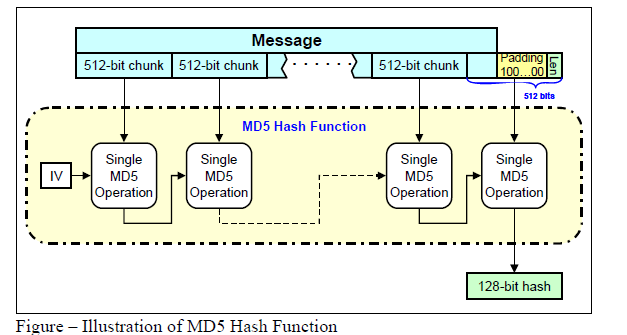
\includegraphics[scale=.65]{md5.png}

\subsection{L'algorithme MD5}
Le processus de fonctionnement de MD5 peut être décrite dans les étapes suivantes.
\begin{enumerate}
\item {\it{le padding}}. Si la longueur du message n'est pas un multiple de 512, on ajoute un pad, dont le premier bit est à 1 suivi de 0 de telle sorte que la longueur résultante soit égale à 448 mod 512. Cette valeur est choisi pour pouvoir ajouter derrière ce padding un la longueurd du message original pour avoir une longueur de message multiple de 512 ;
\item {\it{le partitionnement}}. MD5 découpe le message original résultant d'un padding ou non en N blocs de 512 bits ;
\item {\it{le processus}}. MD5 calcule des valeurs intermémdiaire de hash, {\it{IHV}}. Chaque IHV consiste à utiliser 4 mots de 32 bits comme vu dans la section précédente. (a0, b0, c0, d0) sont des valeurs publiques fixées, et pour chaque IHV calculé en utilisant la fonction de compression MD5Compress telle que: IHV(i) = MD5(IHV(i-1), M(i)) ;
\item {\it{le résultat}}. La valeur du hash résultant est la dernière valeur IHV calculée. Cet IHV est la concaténation en hexadécimal des derniernes valeurs (a, b, c, d) calculés.
\end{enumerate}


\subsection{La fonction de compression MD5Compress}
MD5Compress(IHV, B) est la focntion de compression de MD5. Elle prend en entrée des valeur de hachage intermédiaire appelées IHV, et un block de message B de taille 512 bits.\\

Pour calculer le haché la fonction de hachage s'éffectue en 64 étapes. Ces 64 étapes sont découpés en 4 tours de 16 étapes. A chaque étape sont associés les opérations suivantes:
\begin{itemize}
\item addition modulaire;
\item rotation gauche;
\item utilisation d'une fonction non-linéaire ;
\end{itemize}


\section{Localisation de collisions: de la théorie...}
Comme nous l'avons vu dans les chapitres précédent, MD5 s'inspire du modèle de merkle-Damgard pour calculer le haché d'une entrée.

\subsection{Attaques possibles}
La fonction de compression est une fonction détemriniste. Ce qui veut dire qu'à une entrée sera toujours attribuée une même sortie. 

\subsubsection{Attaque par force brute}
Dans ce modèle, il faut essayer toute les combinaisons possibles en essayant toutes les clés possibles sur un text chiffré jusqu'à obtenir une réponse. cette recherche sera très longue, compte tenu de la longueur du message en entrée. .......\\
Une alternative à cette étude est l'attaque à préfixe choisi.


\subsubsection{Attaque à préfixe choisi}

L'attaque à préfixe choisi, est une attaque différentielle dont les principales étapes sont les suivantes:
\begin {enumerate}
 \item Phase de pré-calcul.
 \begin{itemize}
  \item choisir un delta message ;
  \item trouver le différence dans la chaine de blocs ;
  \item calculer un ensemble de conditions suffisant à réduire cette différence ;
 \end{itemize}
 \item Chercher un message M qui satisfait les conditions de collisions; alors on aura MD5(M) = MD5(M + delta).
\end{enumerate}

En d'autre termes, une collision à préfixe choisi est une paire de  message (M, M') dont on à choisi leurs préfixes (P, P') on génère une paire de suffixe (S, S') de telle sorte que l'on ait:
\begin {enumerate}
 \item M = concat(M, S) ou S = concat(Sr, Sb, Sc) avec r = padding, b =  bit d'aniversaite, c = block de collision;
 \item M' = concat(M', S') ou S' idem à S;
 \item MD5(M) = MD5(M') ;
\end{enumerate}

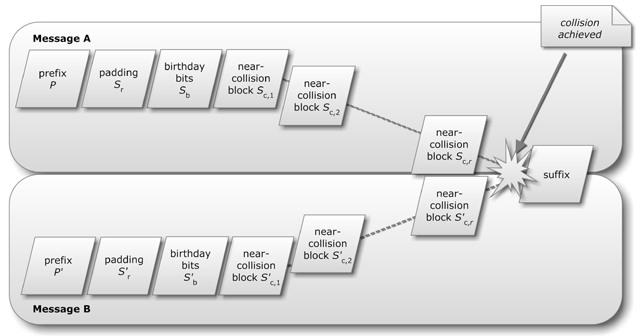
\includegraphics[scale=.65]{collision.png}


\section{\`A la pratique}

\subsection{Première approche}
le but de cette partie est de générer des messages M de 512 bits aléatoire, jusqu'à trouver deux qui ait le même haché H. Le couple (M, H) est la collision.\\
On sait que d'après le théorème des anniversaires, il faut de l'ordre de 2 exp(m/2) messages en moyenne pour trouver une collision pour des hachés de m bits. Dans notre cas, la probabilité de trouver une collision est de 2 exp(256).\\

Dans cette partie, nous allons sauvegarder les couple (M, H) dans une table de hachage. Le choix de l'indice du tableau se porte sur le haché du mot en lui même. En d'autres termes, chaque indice i du tableau est représenté par les 64 premiers bits du haché. Le couple stocké à l'indice i sera alors le message M et les 64 derniers bits du haché.

\subsubsection{L'algorithme de recherche de collision simple}

\begin{algorithm}
\caption{Recherche de collisions simple sur des mots}
\begin{algorithmic} 
\WHILE{pas de collision trouvée}
\STATE Tirer un message aléatoire de 512 bits
\STATE Calculer son haché
\STATE Vérifier si ce haché à déjà été trouvé
\IF{le haché à été trouvé}
\STATE Afficher les 2 messages et leurs hachés
\ELSE
\STATE Inserer le message dans la table de hachage
\ENDIF
\ENDWHILE
\end{algorithmic}
\end{algorithm}

%%==============================

\end{document}